\documentclass[aspectratio=169]{beamer}
\usepackage{will_handley_beamer}
\usepackage{title_page}
\usetikzlibrary{positioning, calc, arrows.meta, shapes}

% Commands
% --------
% - \arxiv{arxiv number}
% - \arxiv{<number>}            arxiv.org/abs/<number>
% - \oldarxiv{<arxiv number>}   arxiv.org/<number>
% - \doi{<doi>}                 doi.org/<doi>
% - \xkcd{<number>}             xkcd.com/<number>
% - \email{<email>}             <<email>>
% - \tthref{<website>}          <website>
% - \av[dist]{<quantity>}       <quantity>_{dist}
% - \student{<name>}{<detail>}{<photo>}

% Talk details
% ------------
\title{GPU-native nested sampling in BlackJAX}
\subtitle{For simulation-based inference at scale}
\date{Bristol SBI Galaxy Evolution Workshop 2025}

\begin{document}

\begin{frame}
    \titlepage
\end{frame}

\begin{frame}
    \frametitle{What is Nested Sampling?}
    \begin{itemize}
        \item Nested sampling is a radical, multi-purpose numerical tool.
        \item Given a (scalar) function $f$ with a vector of parameters $\theta$, it can be used for:
    \end{itemize}
    \vspace{-10pt}
    \begin{columns}[t]
        \column{0.3\textwidth}
        \begin{block}{Optimisation}
            \[\theta_\text{max} = \max_\theta{f(\theta)}\]
        \end{block}
        \column{0.3\textwidth}
        \begin{block}{Exploration}
            \vspace{-10pt}
            \[\text{draw/sample}\quad \theta\sim f\]
            \vspace{-15pt}
        \end{block}
        \column{0.3\textwidth}
        \begin{block}{Integration}
            \[\int f(\theta) dV \]
        \end{block}
    \end{columns}
    \begin{columns}[t]
        \column{0.33\textwidth}
        \centerline{\includegraphics[width=0.8\textwidth,page=13]{figures/himmelblau}}
        \column{0.33\textwidth}
        \centerline{\includegraphics[width=0.8\textwidth,page=15]{figures/himmelblau}}
        \column{0.33\textwidth}
        \centerline{\includegraphics[width=0.8\textwidth,page=14]{figures/himmelblau}}
    \end{columns}
\end{frame}

\begin{frame}
    \frametitle{Why nested sampling for SBI?}
    \begin{columns}
        \column{0.5\textwidth}
        \begin{itemize}
            \item Other than NPE, all SBI methods (NLE, NRE, NJE etc) need a sampler
            \item Most existing samplers are limited:
                \begin{itemize}
                    \item \textbf{Legacy implementations}: MultiNest, PolyChord (Fortran)
                    \item \textbf{Slow Python codes}: dynesty, ultranest, nautilus
                \end{itemize}
            \item BlackJAX solution:
                \begin{itemize}
                    \item GPU-native implementation
                    \item Open source \& community-driven 
                    \item Dissociated from original authors
                \end{itemize}
        \end{itemize}
        \column{0.5\textwidth}
        \centerline{%
            \begin{tikzpicture}[
                    every node/.style={align=center, font=\bfseries},
                    box/.style={draw, rounded corners, minimum width=2cm, minimum height=1cm, fill=C2!30},
                    trapezoid/.style={draw, trapezium, minimum width=2cm, minimum height=1cm, trapezium stretches body, fill=C1!50},
                    ellipsoid/.style={draw, ellipse, minimum width=2cm, minimum height=1cm, fill=C0!50},
                    cloudoid/.style={draw, cloud, cloud puffs=10, aspect=2, inner ysep=1em, fill=C3!30},
                    arrow/.style={thick, -{Stealth[length=3mm, width=2mm]}}
                ]
                \node[ellipsoid] (theory) {\Large Theory};
                \node[trapezoid] (experiment) at (6,0) {\Large Experiment};
                \node[box] (forward) at (3,1.5) {Forward Model};
                \node[cloudoid] (inference) at (3,-1.5) {Inference};
                \draw[arrow] (theory) to[bend left=25]  (forward);
                \draw[arrow] (forward) to[bend left=25] (experiment);
                \draw[arrow] (experiment) to[bend left=25] (inference);
                \draw[arrow] (inference) to[bend left=25] (theory);
            \end{tikzpicture}
        }
    \end{columns}
\end{frame}

\begin{frame}
    \frametitle{The GPU imperative}
    \begin{columns}
        \column{0.6\textwidth}
        \begin{itemize}
            \item The future is GPU, whether we like it or not:
                \begin{itemize}
                    \item All future HPC heavily weighted toward GPUs
                    \item Driven by machine learning adoption
                    \item Low-power ARM-based GPUs becoming the norm
                \end{itemize}
            \item JAX does two \emph{separate} things:
                \begin{enumerate}
                    \item \textbf{Automatic differentiation}
                    \item \textbf{Just-in-time compilation} for GPUs
                \end{enumerate}
            \item People often conflate these - they are separate and glorious!
            \item Alternative tools (harmonic, floz) get strength from GPU, not sampling method
        \end{itemize}
        \column{0.4\textwidth}
        \begin{block}{GPU ecosystem growth}
            \begin{description}
                \item[CMB] \texttt{cosmopower}, \texttt{candl}
                \item[SNe] \texttt{BayesSN}
                \item[GW] \texttt{ripple}, \texttt{jim}
                \item[EP] \texttt{ExoJAX}
            \end{description}
        \end{block}
        \github{JAXtronomy}
    \end{columns}
\end{frame}

\begin{frame}
    \frametitle{BlackJAX nested sampling}
    \student{david_yallup}{David Yallup}{PDRA}
    \begin{columns}
        \column{0.6\textwidth}
        \begin{itemize}
            \item Very recent work (past month!)
            \item Nested slice sampler in BlackJAX
            \item Think MultiNest for JAX
            \item Plugs into \texttt{jim} and \texttt{ripple}
            \item Installation:
        \end{itemize}
        \begin{block}{Installation}
            \texttt{pip install git+https://github.com/handley-lab/blackjax@nested\_sampling}
        \end{block}
        \begin{block}{Usage}
            \texttt{import blackjax.ns.adaptive}
        \end{block}
        \column{0.4\textwidth}
        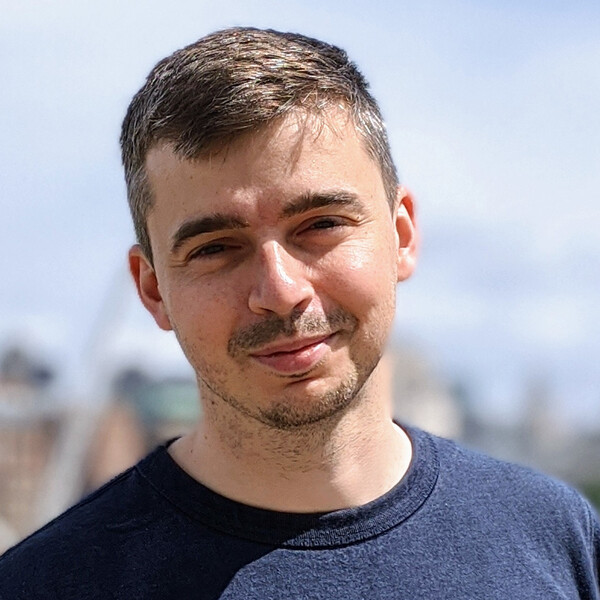
\includegraphics[width=\textwidth]{people/david_yallup.jpg}
    \end{columns}
\end{frame}

\begin{frame}
    \frametitle{The AI surge in scientific research}
    \begin{columns}
        \column{0.7\textwidth}
        \begin{itemize}
            \item We are witnessing an unprecedented AI acceleration in scientific computing:
                \begin{itemize}
                    \item GPU-accelerated inference becoming standard
                    \item Large language models facilitating code development
                    \item Neural networks powering SBI methods
                    \item Automatic differentiation enabling new sampling techniques
                \end{itemize}
            \item This workshop and talk preparation itself demonstrates the AI revolution:
                \begin{itemize}
                    \item Writing and organizing this content in one day
                    \item AI-assisted research workflows
                    \item Community-driven development models
                \end{itemize}
            \item BlackJAX represents this new paradigm: \textbf{open, fast, and AI-ready}
        \end{itemize}
        \column{0.3\textwidth}
        \begin{block}{Key advantages}
            \begin{itemize}
                \item Performance at scale
                \item Community development
                \item Modern software practices
                \item Integration ready
            \end{itemize}
        \end{block}
    \end{columns}
\end{frame}

\begin{frame}
    \frametitle{Workshop goals}
    \begin{columns}
        \column{0.5\textwidth}
        \begin{itemize}
            \item Today we'll explore:
                \begin{enumerate}
                    \item Running nested sampling with BlackJAX
                    \item Visualization with Anesthetic
                    \item Performance comparison: nested sampling vs AIES
                    \item Integration with your JAX workflows
                \end{enumerate}
            \item Hands-on notebook environment
            \item Google Colab compatible
            \item Build on Viraj's JAX/SciML workshop
        \end{itemize}
        \column{0.5\textwidth}
        \begin{block}{Links}
            \begin{itemize}
                \item BlackJAX: \github{handley-lab/blackjax}
                \item Anesthetic: \tthref{anesthetic.readthedocs.io}
                \item Workshop materials: \github{handley-lab}
            \end{itemize}
        \end{block}
        \vspace{10pt}
        \begin{alertblock}{Performance promise}
            Compare BlackJAX nested sampling performance with traditional tools and see the GPU advantage firsthand!
        \end{alertblock}
    \end{columns}
\end{frame}

\begin{frame}
    \frametitle{Conclusions}
    \framesubtitle{\github{handley-lab}}
    \tikz[overlay,remember picture]
        \node[anchor=north east] (A) at ($(current page.north east)+(0,0)$) {
        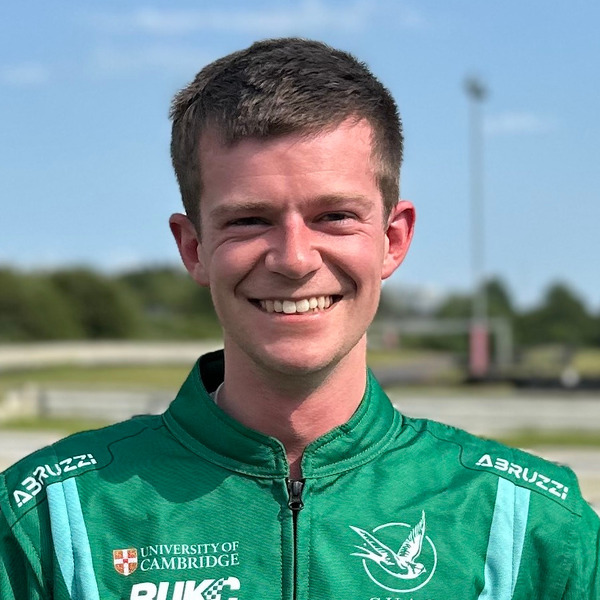
\includegraphics[width=0.09\textheight]{people/adam_ormondroyd.jpg}%
        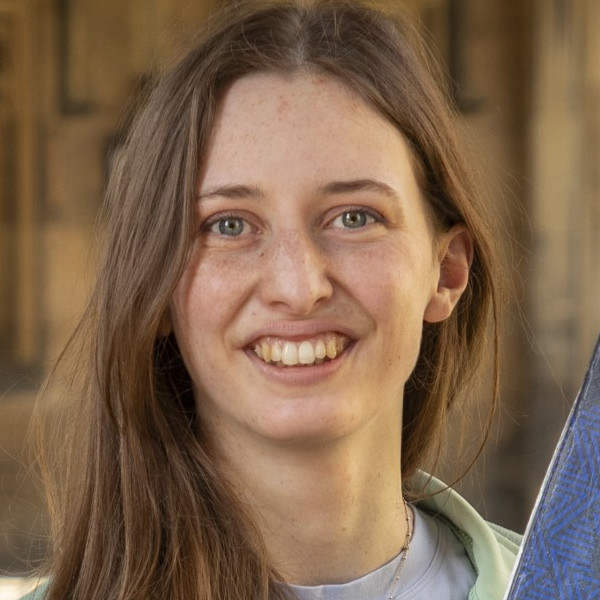
\includegraphics[width=0.09\textheight]{people/charlotte_priestley.jpg}%
        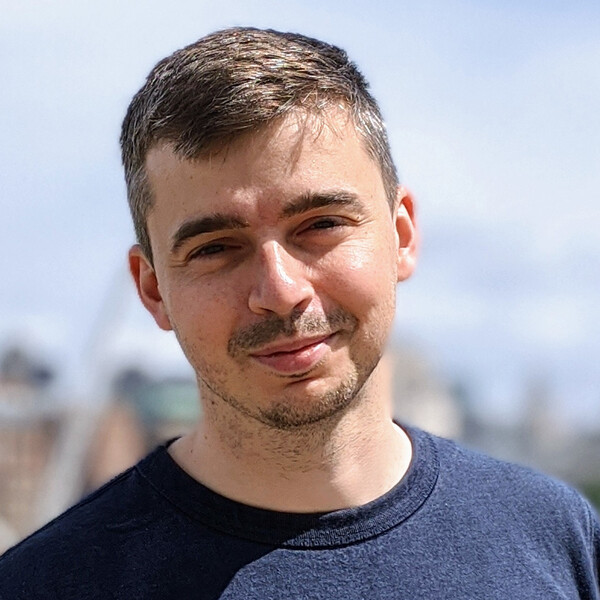
\includegraphics[width=0.09\textheight]{people/david_yallup.jpg}%
        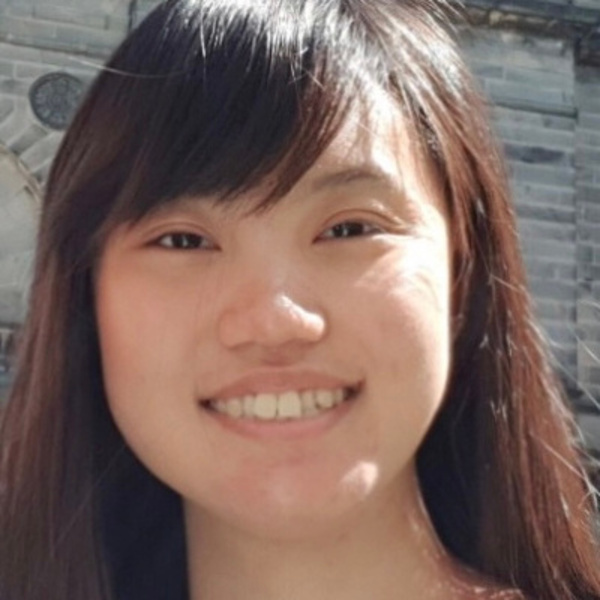
\includegraphics[width=0.09\textheight]{people/dily_ong.jpg}%
        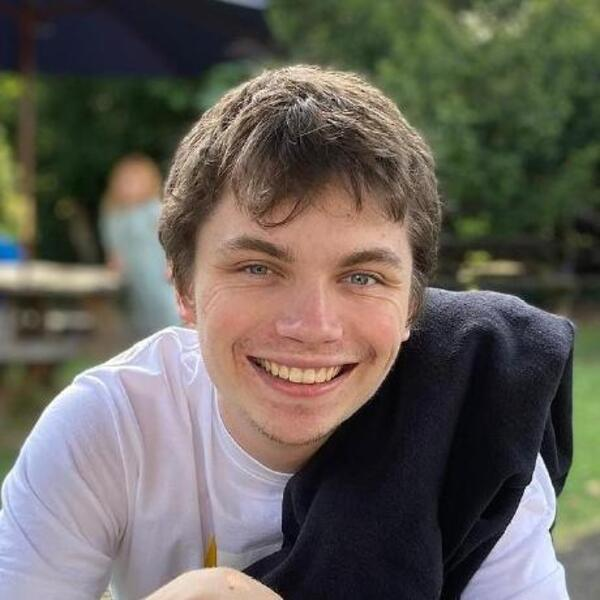
\includegraphics[width=0.09\textheight]{people/harry_bevins.jpg}%
        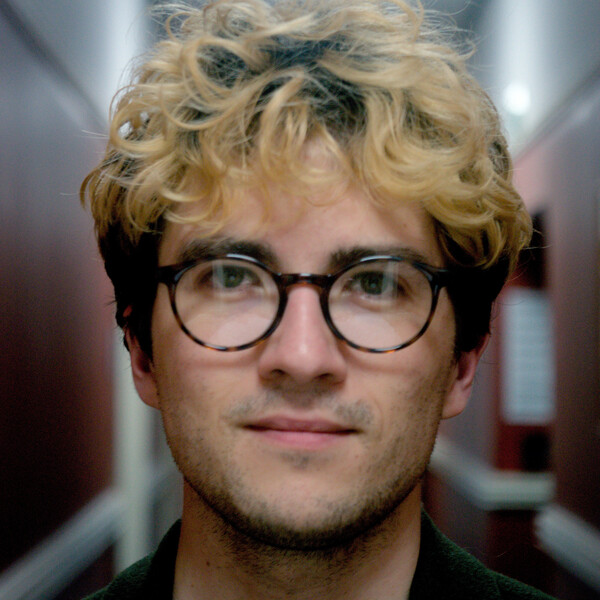
\includegraphics[width=0.09\textheight]{people/harvey_williams.jpg}%
        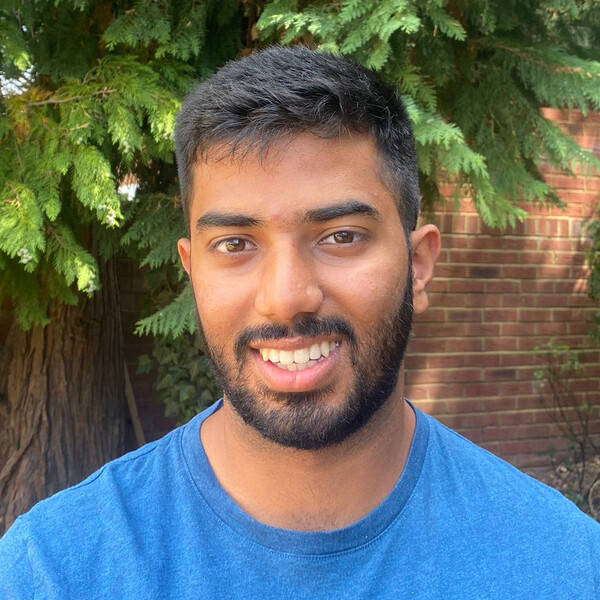
\includegraphics[width=0.09\textheight]{people/krish_nanavati.jpg}%
        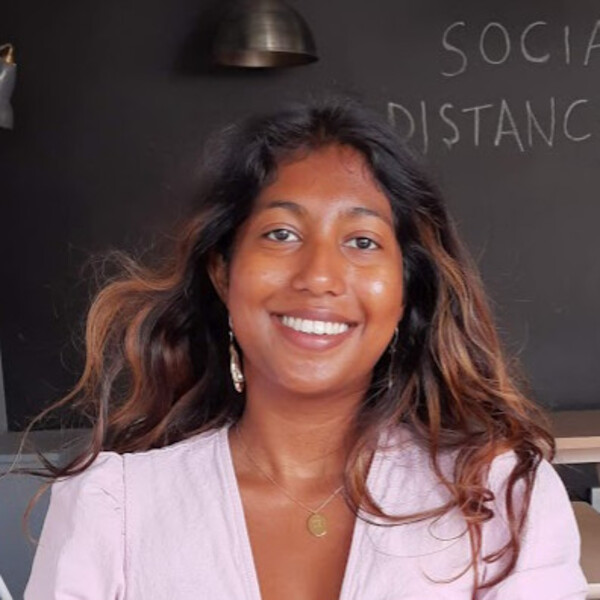
\includegraphics[width=0.09\textheight]{people/metha_prathaban.jpg}%
        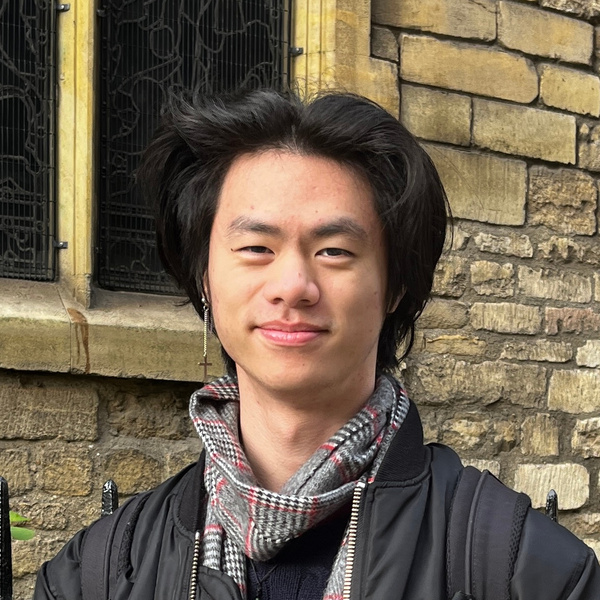
\includegraphics[width=0.09\textheight]{people/ming_yang.jpg}%
        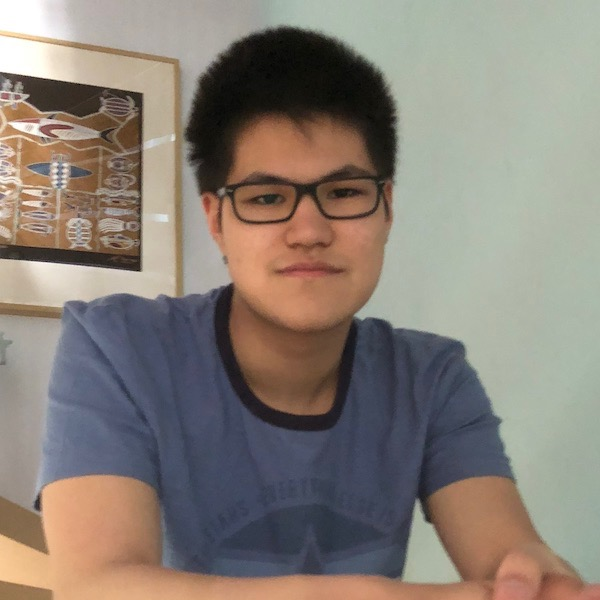
\includegraphics[width=0.09\textheight]{people/namu_kroupa.jpg}%
        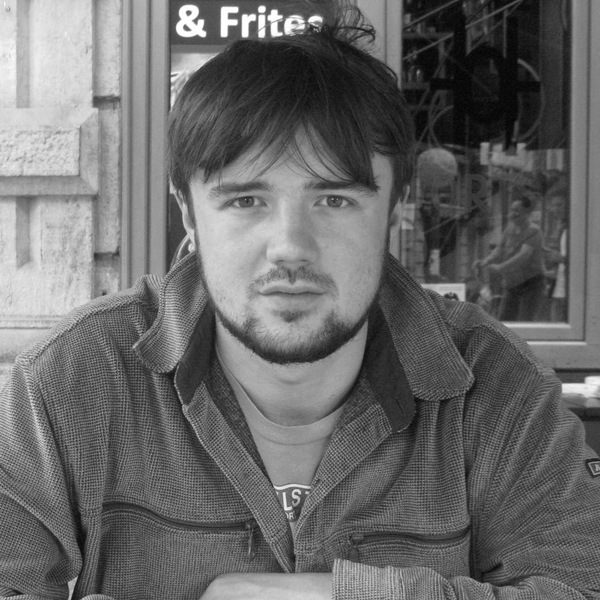
\includegraphics[width=0.09\textheight]{people/sam_leeney.jpg}%
        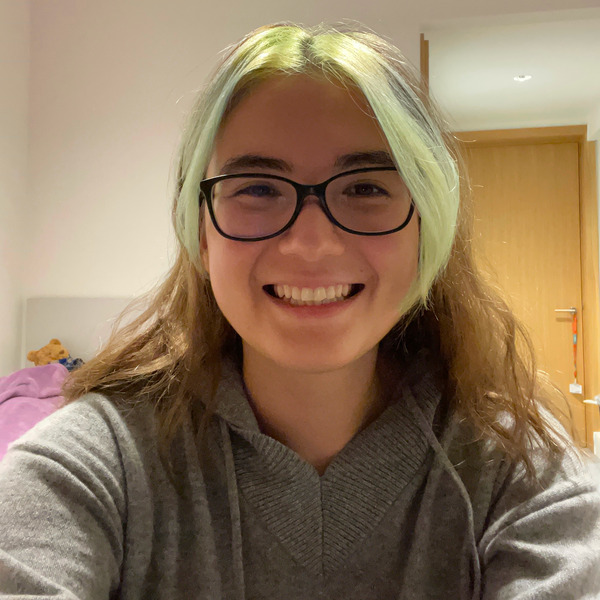
\includegraphics[width=0.09\textheight]{people/sinah_legner.jpg}%
        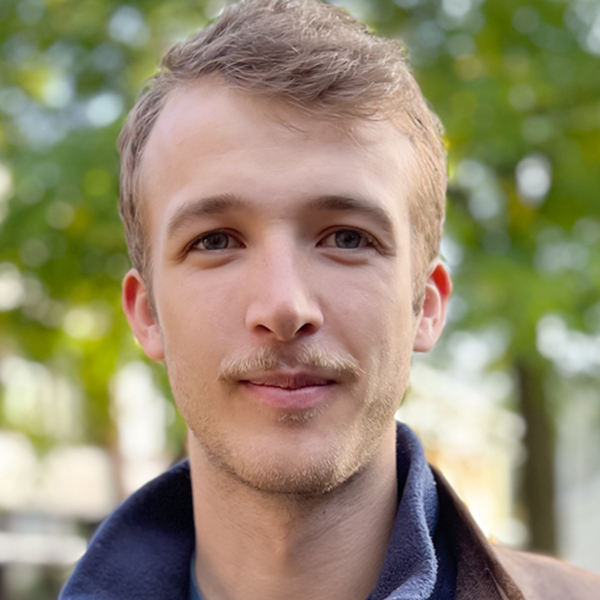
\includegraphics[width=0.09\textheight]{people/toby_lovick.jpg}%
        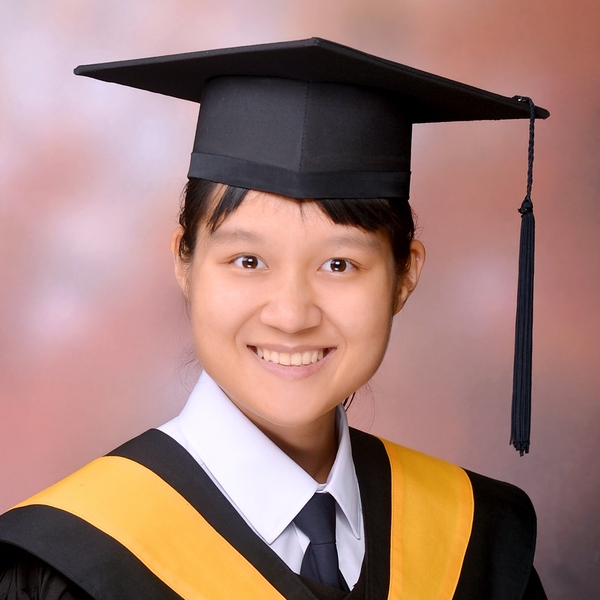
\includegraphics[width=0.09\textheight]{people/wei-ning_deng.jpg}%
        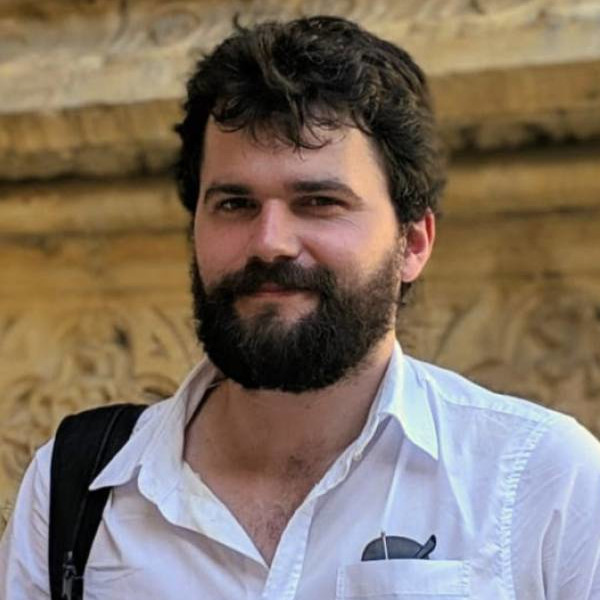
\includegraphics[width=0.09\textheight]{people/will_handley.jpg}%
        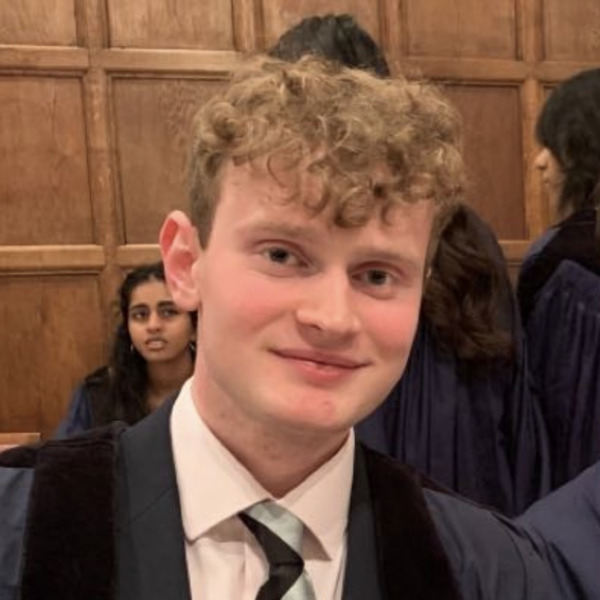
\includegraphics[width=0.09\textheight]{people/will_templeton.jpg}%
    };
    \vspace{-0.1\textheight}
    \begin{itemize}
        \item \textbf{Nested sampling is essential} for most SBI methods (except NPE)
        \item \textbf{BlackJAX} provides GPU-native, community-driven implementation
        \item \textbf{JAX's dual power}: autodiff + JIT compilation for unprecedented performance
        \item \textbf{The future is GPU-accelerated} scientific computing with AI integration
    \end{itemize}
\end{frame}

\appendix

\begin{frame}
    \frametitle{Integration in Physics}
    \begin{itemize}
        \item Integration is a fundamental concept in physics, statistics and data science:
    \end{itemize}
    \begin{columns}
        \column{0.3\textwidth}
        \begin{block}{Partition functions}
            \vspace{-11pt}
            \[ Z(\beta) = \int e^{-\beta H(q,p)} dq dp \]
        \end{block}
        \column{0.3\textwidth}
        \begin{block}{Path integrals}
            \[ \Psi = \int e^{i S} \mathcal{D}x \]
        \end{block}
        \column{0.3\textwidth}
        \begin{block}{Bayesian marginals}
            \vspace{-11pt}
            \[ \mathcal{Z}(D) = \int \mathcal{L}(D|\theta) \pi(\theta) d\theta \]
        \end{block}
    \end{columns}
    \begin{columns}
        \column{0.6\textwidth}
        \begin{itemize}
            \item Need numerical tools if analytic solution unavailable.
            \item High-dimensional numerical integration is hard.
            \item Riemannian strategy estimates volumes geometrically:
                \[ \int f(x) d^nx \approx \sum_i f(x_i) \Delta V_i \sim \mathcal{O}(e^n) \]
            \item Curse of dimensionality $\Rightarrow$ exponential scaling.
        \end{itemize}
        \column{0.4\textwidth}
        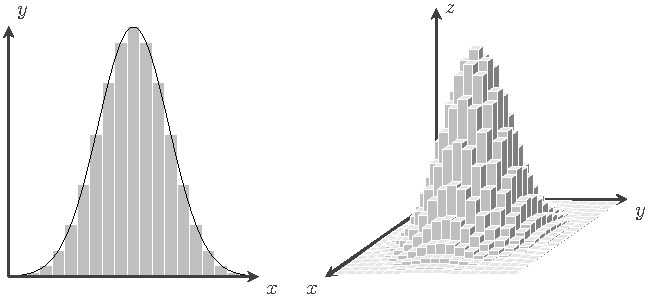
\includegraphics[width=\textwidth]{figures/integration}
    \end{columns}
\end{frame}

\begin{frame}
    \frametitle{MCMC vs Nested Sampling}
    \begin{columns}
        \column{0.48\textwidth}
        \begin{block}{\textbf{MCMC}}
            \begin{itemize}
                \item Single ``walker''
                \item Explores posterior
                \item Fast, if proposal matrix is tuned
                \item Parameter estimation, suspiciousness calculation
                \item Channel capacity optimised for generating posterior samples
            \end{itemize}
        \end{block}
        \centerline{\includegraphics[width=0.5\textwidth,page=19]{figures/himmelblau}}
        \column{0.48\textwidth}
        \begin{block}{\textbf{Nested sampling}}
            \begin{itemize}
                \item Ensemble of ``live points''
                \item Scans from prior to peak of likelihood
                \item Slower, no tuning required
                \item Parameter estimation, model comparison, tension quantification
                \item Channel capacity optimised for computing partition function
            \end{itemize}
        \end{block}
        \centerline{\includegraphics[width=0.5\textwidth,page=4]{figures/himmelblau}} 
    \end{columns}
\end{frame}

\begin{frame}
    \frametitle{The nested sampling meta-algorithm: live points}
    \begin{columns}
        \column{0.5\textwidth}
        \begin{itemize}
            \item Start with $n$ random samples over the space.
            \item Delete outermost sample, and replace with a new random one at higher integrand value.
            \item The ``live points'' steadily contract around the peak(s) of the function.
            \item We can use this evolution to estimate volume \emph{probabilistically}.
            \item At each iteration, the contours contract by $\sim\frac{1}{n}$ of their volume.
            \item This is an exponential contraction, so
                \[  \int f(x) dV \approx \sum_i f(x_i) \Delta V_i, \quad V_i = V_0 e^{-i/n} \]
        \end{itemize}
        \column{0.5\textwidth}
        \includegraphics[width=\textwidth,page=4]{figures/himmelblau}
    \end{columns}
\end{frame}

\begin{frame}
    \frametitle{Types of nested sampler}
    \begin{itemize}
        \item Broadly, most nested samplers can be split into how they create new live points.
        \item i.e. how they sample from the hard likelihood constraint $\{\theta\sim \pi : \mathcal{L}(\theta)>\mathcal{L}_* \}$.
    \end{itemize}
    \vspace{-10pt}
    \begin{columns}[t]
        \column{0.48\textwidth}
        \begin{block}{Rejection samplers}
            \begin{itemize}
                \item e.g. \texttt{MultiNest}, \texttt{UltraNest}.
                \item Constructs bounding region and draws many invalid points until $\mathcal{L}(\theta)>\mathcal{L}_*$.
                \item Efficient in low dimensions, exponentially inefficient $\sim\mathcal{O}(e^{d/d_0})$ in high $d>d_0\sim10$.
            \end{itemize}
        \end{block}
        \column{0.48\textwidth}
        \begin{block}{Chain-based samplers}
            \begin{itemize}
                \item e.g. \texttt{PolyChord}, \texttt{ProxNest}.
                \item Run Markov chain starting at a live point, generating many valid (correlated) points.
                \item Linear $\sim\mathcal{O}(d)$ penalty in decorrelating new live point from the original seed point.
            \end{itemize}
        \end{block}
    \end{columns}
    \vspace{5pt}
    \begin{itemize}
        \item Nested samplers usually come with:
            \begin{itemize}
                \item \emph{resolution} parameter $n_\mathrm{live}$ (which improve results as $\sim\mathcal{O}(n_\mathrm{live}^{-1/2})$).
                \item set of \emph{reliability} parameters, which don't improve results if set arbitrarily high, but introduce systematic errors if set too low.
                \item e.g. \texttt{Multinest} efficiency \texttt{eff} or \texttt{PolyChord} chain length $n_\mathrm{repeats}$.
            \end{itemize}
    \end{itemize}
\end{frame}

\end{document}